% !TEX root = BA-Bericht.tex
\chapter{Stand der Technik}\label{ch:StandDerTechnik}
% Auch "Stand der Forschung" oder "Stand der Praxis"

% Bezogen auf die eigenen Zielsetzungen und Fragestellungen soll aufgezeigt werden, wie andere
% dieses oder ähnliche Probleme gelöst haben. Worauf können Sie aufbauen, was müssen Sie neu
% angehen? Wodurch unterscheidet sich Ihre Lösung von anderen Lösungen? Für wissenschaftlich
% orientierte Arbeiten sei hier explizit auf (Balzert, S. 66 ff) verwiesen.



\section{Technologische Grundlagen}
% TODO Wichtige technologischen Grundlagen / Wissenswertes

\subsection{Privatsphäre und Anonymität}

Im diva.exchange Netzwerk sollen digitale Güter austauscht werden können.
Dies ohne sich zu kennen und ohne sich gegenseitig Vertrauen zu müssen.
die Privatsphäre der Teilnehmer geschützt werden.


Der Begriff Anonymität ist oft negativ behaftet.
Unter dem Deckmantel der Anonymiät
Jedoch gibt es auch 

Anonymität und Privatsphäre ist nicht das gleiche.

Wobei

Jedoch kann durch Anonymität die Privatsphäre geschützt werden.
Auch ist Anonymität wichtig für Whistle-Blower und für Leute die unter totalitären Regimen.

\subsection{Anonymisierungs-Netzwerke}

Es gibt eine vielzahl an verschiedenen Anonymisierungsnetzwerken, wobei \glstext{tor} (\glsname{tor}) wahrscheinlich das bekannteste und meist genutzte ist.

In dieser Arbeit wird aber lediglich das Anonymisierungsnetzwerk \glsname{i2p} behandelt und nicht weiter auf andere Anonymisierungsnetzwerke eingegangen, da dieses das Netzwerklayer von diva.exchange darstellt.


\subsection{Das Anonymitätstrilemma}\label{sec:anonymitytrilemma}

Beim Design eines anonymen Kommunikationsprotokoll gibt es grundsätzliche Einschränkungen. Es gilt die folgenden drei Aspekte abzuwägen :

\begin{itemize}
    \item Der Anonymitätsgrad von Sender und Empfänger einer Nachricht
    \item Die benötigte Netzwerkbandbreite
    \item Die Latenzzeiten der Nachrichten
\end{itemize}


Dabei ist es nicht möglich ein Protokoll zu designen, welches einen hohen Anonymitätsgrad bietet, wenig Netzwerkbandbreite benötigt und tiefe Latenzzeiten vorweist.
Die Anonymität geht also immer auf Kosten von höherer Latenzzeiten und/oder mehr benötigter Netzwerkbandbreite (siehe auch Abbildung~\fullref{fig:anonimitytrilemma}).

\begin{figure}[H]
    \centering
    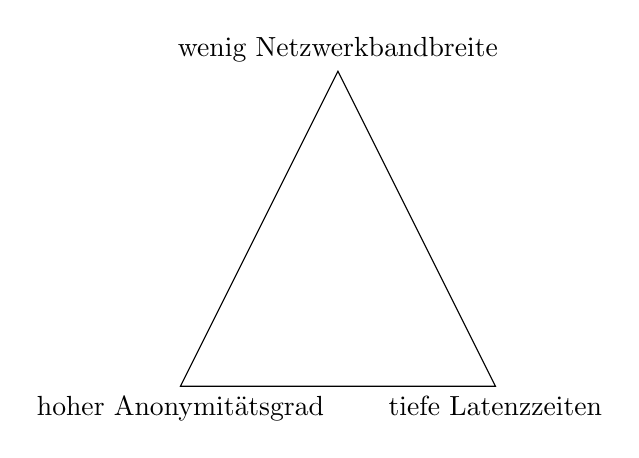
\begin{tikzpicture}
      \draw (0,0) node[anchor=north]{hoher Anonymitätsgrad}
        -- (4,0) node[anchor=north]{tiefe Latenzzeiten}
        -- (2,4) node[anchor=south]{wenig Netzwerkbandbreite}
        -- cycle;
    \end{tikzpicture}
    \caption{Das Anonymitätstrilemma}\label{fig:anonimitytrilemma}
\end{figure}

Ein Anonymisierungsnetzwerk könnte beispielsweise auf Kosten der Netzwerkbandbreite implementiert werden, indem die Nachrichten jeweils an alle Netzwerkteilnehmer versendet werden.
Somit könnte mindestens der Empfänger verschleiert werden.
Umgekehrt könnte ein Anonymisierungsnetzwerk auf Kosten der Latenz implementiert werden. Wenn Nachrichten über mehrere Netzwerkknoten geleitet werden, könnte man Empfänger und Sender verschleiern, aber hätte höhere Latenzzeiten da dieselbe Nachricht mehrmals nacheinander von verschiedenen Netzwerkknoten bearbeitet werden muss.
Letzteres gibt es Netzwerke bei welchen Anonymität keine Rolle spielt, wie beispielsweise beim üblichen UDP Protokoll. Es ist dann möglich hohe Bandbreite sowie niedrige Latenzzeiten zu erreichen.

Es gilt abzuwägen, welche der Aspekte für das zu designende Protokoll wichtig sind und wo ein Schwerpunkt gelegt wird und welche Aspekte somit auch vernachlässigt werden, um einen guten Kompromiss zu finden. \parencite{das_anonymity_2018}

\subsection{\glstext{i2p} (\glsname{i2p})}

Kurz gesagt ist \glstext{i2p} (\glsname{i2p}) ein dezentrales Mischnetzwerk mit niedriger Latenz indem verschlüsselte Nachrichten ausgetauscht werden können.
\parencite{zantout_i2p_2011}
Es handelt sich hier um ein eigenständiges Overlay-Netzwerk, welches auf den darunterliegenden Protokollen UDP und TCP aufbaut.  \parencite{de_boer_invisible_2019,astolfi_i2p_2015}.

Mit einem Mischnetzwerk ist gemeint, dass Nachrichten an durch Knoten des Netzwerks weitergeleitet werden, um den Sender und den Empfänger einer Nachricht zu verschleiern. Dieser Mischvorgang wird bei I2P Garlic-Routing genannt.
\parencite[S.~1]{zantout_i2p_2011}.

Auch gilt es zu unterstreichen, dass \textit{Nachrichten} ausgetauscht werden.
I2P ist \textit{Nachrichtenbasiert} und verhält sich in diesem Sinne ähnlich wie UDP.
Es gibt dementsprechend keine Garantien, dass wenn eine Nachricht versendet wird, dass die Daten in der richtigen Reihenfolge, komplett oder überhaupt ankommen.
Es gibt jedoch Erweiterungen auf dem Netzwerk, welche diese Garantien (ähnlich wie sie diese bei TCP gibt) wieder herstellen können.
Zudem bietet I2P eine Ende-zu-Ende-Verschlüsselung von Nachrichten.
Die Nachrichten sind also vom Sender bis zum Empfänger verschlüsselt.

Während das TOR-Netzwerk ursprünglich entwickelt wurde auf das öffentliche Internet via Out-Proxies zuzugreifen,
liegt bei I2P der Fokus darin anonym auf Dienste, die innerhalb des Netzwerks angeboten werden, zuzugreifen.
Jedoch besteht bei TOR ebenfalls die Möglichkeit netzwerkinterne Dienste anzubieten mittels TOR Hidden Services, auch aber gibt es bei I2P die Möglichkeit, mit Hilfe von sogenannten Outproxies, auf das normale Internet zuzugreifen.

Dienste die innerhalb des Netzwerks angeboten werden, sind zum Beispiel Bit-Torrent für File-Sharing, Webseiten (sogenannte ``eepsites''), oder auch Chat-Dienste wie IRC (Internet Relay Chat).
\parencite[p.~3-4]{de_boer_invisible_2019}

\cite{astolfi_i2p_2015}

\cite{timpanaro_birds_2012}

\cite{timpanaro_evaluation_2015}

A scaleable framework for anonymous communication
\cite{noauthor_i2p_nodate-8}


\cite{hoang_measuring_2019}
\cite{hoang_empirical_2018}

\cite{de_boer_invisible_2019}


\subsection{I2P Router}

Ein I2P-Router ist ein einzelner Teilnehmer oder auch ein Knoten im I2P-Netzwerk.
Ein Router kann einerseits Nachrichten weiterleiten und diese somit im Netzwerk mischen, aber auch Nachrichten empfangen, oder diese versenden.

Es gibt zwei verschiedene Implementationen von I2P-Routern.
Der ursprüngliche Implementation des I2P-Router wurde in Java Implementiert.

In dieser Arbeit wird jedoch lediglich die später entwickelte und schlankere C++-Implementation auch genannt \lstinline|i2pd| (Invisible Internet Protocol Daemon) untersucht. (\cite{noauthor_i})


\section{Technische Konzepte}
\label{sec:technischeKonzepte}
% TODO Konzepte in diesem Feld welche für den Leser relevant sind

In diesem Abschnitt gehen wird nun genauer auf I2P spezifische Begrifflichkeiten Eingegangen und erklärt die I2P technisch funktioniert.

\subsection{NetDb}

Da I2P dezentral und verteilt ist, jedoch aber trotzdem Daten zwischen den Knoten geteilt werden müssen wird eine Art verteilte Datenbank benötigt.
Diese verteilte Netzwerkdatenbank wird NetDb genannt.
Es handelt sich hier um eine \glstext{dht} (\glsname{DHT}) basierend auf dem Kademlia-Algorithmus.

Nur sogenannte Floodfill-Router 
\parencite[S.~5-6]{timpanaro_monitoring_nodate}


kurz NetDb. Eine DHT wo jeder Knoten
Informationen über seine Peers (u.a. Router-Infos) ablegt.

\cite[noauthor_network_nodate]



\subsubsection{Router-Info}

Eine RouterInfo Datei beinhaltet den öffentlichen Schlüssel und die Netzwerkkoordinaten eines einzelnen I2P-Routers.
Jeder I2P-Router erstellt diese Datei beim Aufstarten, falls diese noch nicht vorhanden ist.
Beim erstellen dieser Datei wird auch ein Schlüsselpaar generiert, damit der öffentliche Schlüssel in die Datei abgelegt werden kann.
Zusätzlich werden auch die öffentlichen IP-Addressen ermittelt sowie zufällige Ports ausgewählt über welche der I2P-Router erreicht werden kann.

Diese Informationen werden benötigt damit ein anderer I2P-Router die Kommunikation mit dem I2P-Router aufnehmen kann, der die RouterInfo-Datei erstellt hat.
Anhand der Netzwerkoordinaten (IPv4 und IPv6 Adressen, sowie Ports) ist bekannt wohin eine Anfrage zur Tunnelerstellung gesendet werden muss.
Mit Hilfe des öffentlichen Schlüssels kann die Anfrage zur Tunnelerstellung auch bereits schon Verschlüsselt werden.

% TODO: reference Router info

Es gilt zu erwähnen, die öffentlichen IP-Adressen eines I2P-Knotens somit nicht geheim sind.
Jeder der einen Knoten betreibt, oder einfach nur die NetDb eines Floodfill-Routers anfragt, kann somit  
I2P wurde dazu auch nicht designt. Es wurde designt wurde das Teilnnehmer Nachrichten innerhalb des Netzwerks austauschen 

Ein Beobachter kann also herausfinden, ob ein Rechner am I2P-Netzwerk beteiligt ist, kann jedoch nicht aussagen, ob eine Nachricht für den Knoten bestimmt ist, ob er eine Nachricht versendet, oder ob er diese lediglich weiterleitet.

% TODO: reference FAQ question


\subsubsection{LeaseSet's und Destinations}

Um nun Services auf dem I2P-Netzwerk zur Verfügung zu stellen werde benötigt 

Ein LeaseSet ist eine Sammlung von Tunnel-Eingangspunkten (auch Leases genannt) für eine bestimmte Destination


Um Tunnels miteinander zu Verbinden werden LeaseSet's benötigt. Diese Verbinden ein Out-und Inbound tunnel miteinander. \cite{noauthor_intro_nodate}

\subsection{Tunnels}

Wenn man im Bereich vom Netzwerken über Tunneling-Redet geht es immer Darum ein Kommunikationsprotokoll in ein anderes einzubetten. \cite{noauthor_duden_nodate}
Im I2P ist ein Tunnel ein Kommunikationsweg durch eine ausgewählte Liste an I2P-Routern.

Ähnlich wie beim Onion-Routing wird hier die Nachricht mehrfach verschlüsselt, damit die Zwischenknoten nicht in die Nachricht hineinsehen können, jedoch trotzdem die benötigen Routing-Informationen haben, um diese an den richtigen Ort weiterzuleiten.

\cite{noauthor_intro_nodate}

Um nun auf Basis von IP ein Overlaynetzwerk zu bilden werden in I2P-Verschlüsselte Tunnels verwendet ähnlich wie dies beim Onion-Routing der Fall ist.


Bei I2P gibt es verschiedene Arten von Tunnels, welche in den folgenden Abschnitten genauer differenziert werden.

\subsubsection{Inbound- und Outbound-Tunnels}
Jeder I2P-Router kann eine beliebige Anzahl Inbound- und Outbound Tunnels erstellen.
Wobei die Inbound-Tunnels zum Empfang und die Outbound-Tunnels zum Versand von Nachrichten dienen.
\cite{noauthor_intro_nodate}

    \item \textbf{Inbound-Tunnels}: Diese dienen zum Empfang vom Nachrichten.
    \item \textbf{Outbound-Tunnels}: Diese dienen zum Versand vom Nachrichten.
    \item Exploratory Tunnels

\cite{noauthor_intro_nodate}

\subsubsection{Exploratory--Tunnels}

Exploratory-Tunnels werden dazu verwendet Tunnels aufzubauen.
Um Tunnels zu aufzubauen werden Exploratory-Tunnels verwendet.

Client-Tunnels haben jeweils immer eine Destination. Diese Destination ist innerhalb des I2P-Netzwerks ansprechbar mit einer Netzwerkinternen-Adresse.

\cite{de_boer_invisible_2019}

\subsubsection{Client-Tunnels}

Um Services über das I2P-

Für jedes Client-Tunnel gibt kann es eines oder mehrere LeaseSets geben.


%TODO: inbound outbound nicht verwechseln

\subsubsection{Länge der Tunnels}

Jedes Tunnel hat eine Länge.
Diese gibt an durch wie viele Knoten eine Nachricht, die durch das Tunnel verschickt wird, geroutet wird.
Für jeden Hop im Tunnel wird die Nachricht eine zusätzliche Verschlüsselungsschicht eingehüllt. (vgl. Onion Routing)
Somit wissen die Router jeweils nur Bescheid von welchem anderen Router sie eine Nachricht erhalten haben und an welchen Router die Nachricht weitergeleitet werden soll.
Ein Router im Tunnel weiss also schlussendlich nie von wem an wen eine Nachricht verschickt wurde.

Die Länge eines Tunnels kann auch \lstinline|0| betragen.
In diesem Fall wird eine Nachricht die durch das Tunnel verschickt wird, durch keine weitere Knoten geroutet.

Hierbei kann jeder Knoten selber festlegen wie lange diese Tunnels sind.

Je Länger ein Tunnel ist, desto mehr Anonymität bietet dieser.
Jedoch geht dies auf Kosten der Latenz aufgrund der zusätzlichen Hops.

Tunnels Configuration
\cite{noauthor_i2p_nodate-3}


\begin{itemize}
    \item Jeder Knoten kann die länge seiner Tunnel selber bestimmen. (Standardwert 2)
    \item Mehrere Verschlüsselungsschichten je nach Tunnellänge (vgl. Onion-Routing)
\end{itemize}

\subsection{Garlic-Routing}

Inspiriert vom Onion-Routing des \glsname{tor}-Netzwerk's gibt es im I2P-Netzwerk der Begriff

\begin{figure}[H]
    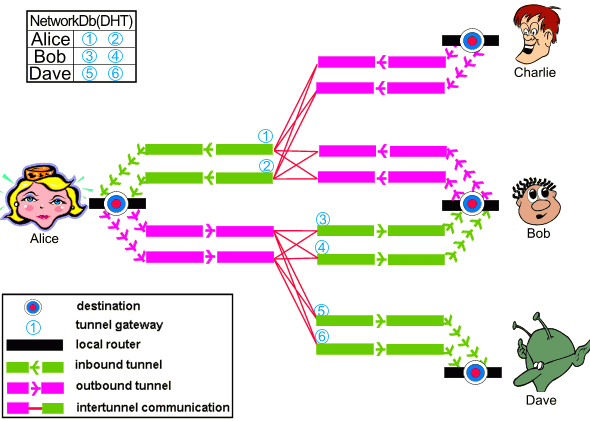
\includegraphics[width=\textwidth]{img/i2prouting.png}
    \caption{Garlic-Routing (vgl. \url{https://geti2p.net/de/docs/how/intro})}
\end{figure}

\begin{itemize}
    \item
\end{itemize}

\cite{de_boer_invisible_2019}

\cite{noauthor_intro_nodate}



\section{Stand im Bezug auf eigenes Projekt}
% TODO Welche Forschung wurde in jüngster Zeit gemacht welche relevant für das eigene Projekt sind

\subsection{Bootstrapping und Reseed-Servers}

Es wird Bootstrapping-Prozess benötigt, dass sich die I2P-Router sich anfangs Gegenseitig im privaten und abgeschotteten Testnetzwerk überhaupt finden können.
Erst anschliessend ist es möglich Tunnels aufzubauen, damit die I2P-Router miteinander kommunizieren können.


Einerseits gibt es hier den Floodfill-Ansatz oder einen eigen Reseed-Server zu im privaten Testnetzwerk zu haben.
%TODO: reference bootstrapping site

Reseed Access
\cite{noauthor_i2p_nodate-7}

Usability Inspection of Anonmity Networks
(\cite{abou-tair_usability_2009})

Usability Tetsts
(\cite{schomburg_anonymity_2009})

Evaluation of Anonymity Networks
(\cite{timpanaro_evaluation_2015})

\subsection{Performance}

In der Vergangenheit wurde schon vielfach an der Performance von I2P gearbeitet.

Es ist jedoch unklar welche der Vorschläge bereits implementiert wurden, weil die Webseiten schon lange nicht mehr aktualisiert wurde.
Zudem könnte es sich hier auch nur um Performance Verbesserungen, welche die Java-Implementation von I2P betreffen aufgelistet sein.
Es ist unklar welche dabei spezifisch in i2pd (der C++ Implementation implementiert wurden).

Während es öffentlich zugängliche Metriken gibt über die 


Performance improvement using SSL IN I2P
\cite{vashi_performance_2015}

Performance I2P Webseite
\cite{noauthor_performance_nodate}

Performance History I2P Webseite
\cite{noauthor_performance_nodate-1}

Auf der Webseite von I2P auf der Seite ''Future Performance Improvements'' sind zudem zukünftige Performance Verbesserungsmöglichkeiten aufgelistet.
\cite{noauthor_future_nodate}

Improving I2P (2012)
\cite{timpanaro_improving_2012}

Latency vs Tor Usability Bandwitdh and Latency Comparision
\cite{ehlert_i2p_2021}


\subsection{Peer-Profiling und Tunnel-Erstellung}

Die einfachste Möglichkeiten Nachbarknoten (oder Peers) zur Tunnelerstellung auszuwählen, wäre zufällig Knoten auszuwählen. 
Jedoch wird dies aus Performanzgründen nicht so gehandhabt.
Jeder I2P-Knoten testet seine Nachbarknoten auf Performanz, Latenzzeiten und ob diese Verfügbar sind und kategorisiert diese.

Natürlich hat dies auch einen Einfluss auf den Anonymitätsgrad.
\parencite[S.~4-5]{timpanaro_monitoring_nodate}

Die Auswahl von welchen Knoten welche für die Tunnelers

Jeder I2P-Knoten


\subsection{Testen mit dem I2P-Netzwerk}

\subsection{Metriken zur Messung}

\begin{itemize}
    \item Latenzmessung (abschicken/empfangen (Laport-Zeitstempel im schlimmsten fall))
    \item Messung der Bandbreite (ab welchem Layer)
    \item Ressourcenauslastung
\end{itemize}

Towards Measuring on the I2P Netzwerk
\cite{wang_towards_2013}


Es sind auch diverse Metriken über das öffentliche \glsname{i2p}-Netzwerk verfügbar auf
Im öffentlichen \glsname{i2p} Es werden bereits verschiedene Dinge gemessen


\cite{timpanaro_monitoring_nodate}

\subsection{Testen im öffentlichen I2P Netzwerk}

\begin{itemize}
    \item family tag \cite{noauthor_family_nodate}
    \item verfälscht resultate
    \item deshalb isolieren
    \item öffentliche Metriken  I2P Metrics: \cite{noauthor_i2p_nodate-4}
    \item Netzwerk ist klein (deshalb braucht es so ein Beweis wie hier)
\end{itemize}

\subsection{Flooding von Blockchain-Updates}

Es werden 64Kb Nachrichten verteilt über verschiedene Knoten.
